\chapter{Procedure} \label{chapter2:Procedure}

Throughout this chapter, assume that we have observed data at $n$ (not necessarily evenly spaced) spatial locations $\{\bm{s}_1, \dots, \bm{s}_n\}$. These locations exist on some bounded domain $\mathcal{D} \subseteq{R}^d$. The data, $\bm{y} =(y_1, \dots, y_n)^T$, are values of the random variables $\bm{Y} = (Y(\bm{s}_1), \dots, Y(\bm{s}_n))^T$, and this is a single realization of a Gaussian process with mean 0 and covariance function $C$. By the definition of Gaussian processes,
\[
	\bm{Y} \sim \mathcal{N}_n(\bm{0}, \bm{\Sigma}).
\]
We aim to estimate the covariance function.

\section{Estimating the Covariance Function} % (fold)
\label{sec:estimating_the_covariance_function}

Under the assumptions of stationarity and isotropy, the $ij$th element is
\[
	\Sigma_{ij} = \textrm{Cov}(y_i, y_j) = C(||\bm{s}_i - \bm{s}_j||) = C(h_{ij}).
\]
Here $h_{ij}$ is the Euclidean distance between locations $\bm{s}_i$ and $\bm{s}_j$. We can use \eqref{eq:bochner2} to obtain an integral representation for each element of $\bm{\Sigma}$.
\begin{equation}
	\Sigma_{ij} = \int \cos(h_{ij}\omega) \; f(\omega) \; d\omega
\end{equation}
Were we able to sample from the spectral density $f(\omega)$, we could estimate $\Sigma_{ij}$ using Monte Carlo integration:
\begin{equation}
	\Sigma_{ij} \approx \widehat{\Sigma}_{ij} = \frac{1}{M} \sum_{m=1}^M \cos(h_{ij}\widetilde{\omega}_m)
\end{equation}
for $M$ samples $\{\widetilde{\omega}_1, \dots, \widetilde{\omega}_M\}$ from $f(\omega)$.

% section estimating_the_covariance_function (end)

\section{Semiparametric Modeling of the Spectral \\ Density} % (fold)
\label{sec:semiparametric_modeling_of_the_spectral_density}

We don't know the exact form of $f(\omega)$, so we will have to estimate it as well in order to generate random samples. Recall that according to Bochner's theorem, $f$ is a symmetric density, so it suffices to restrict our attention to estimating $f(\omega)$ for $\omega > 0$.

Rather than estimating $f(\omega)$ directly, we apply a straightforward variable transformation and estimate $\log f(\log \omega)$ instead. It is easy to show that any density with power law tails has linear tails on the log-log scale. Suppose $f_X(x) = cx^{-b}$, $b > 1$, and let $Y = \log X$. Then
\begin{align*}
	f_Y(y) &= f_X(e^y) \frac{d}{dy}(e^y) \\
	&= ce^{-by}e^y \\
	&= ce^{-(b-1)y},
\end{align*}
and so
\[
	\log f_Y(y) \propto -(b-1)y.
\]
This fact is illustrated further in Figure~\ref{fig:logdens_ex}.

\begin{figure}[!htb]
	\centering
	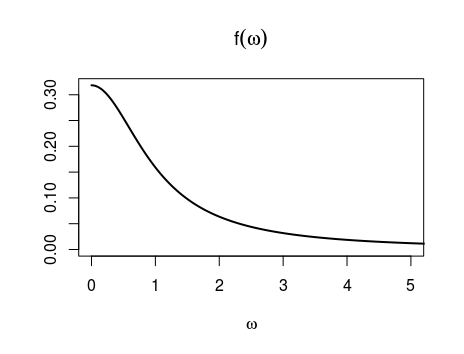
\includegraphics[width=0.48\textwidth]{dens_ex.png}
	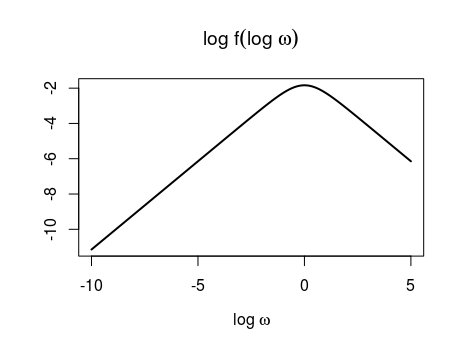
\includegraphics[width=0.48\textwidth]{logdens_ex.png}
	\caption{\small A density $f$ with power law tails (left) and the same density transformed to the log-log scale (right). Both the left and right tails of the transformed density are linear.}
	\label{fig:logdens_ex}
\end{figure}

An important benefit to working in this log-transformed space is that linear tails are ideal for modeling the curve using a natural spline basis, which is constructed to ensure linearity beyond the outermost (\emph{boundary}) knots. If we are willing to assume that the tails of $\log f(\log \omega)$ are truly linear, then fitting it with natural splines will result in a good approximation over then entire domain $\log \omega \in (-\infty, \infty)$ without needing to use a large number of knots.

It might appear that requiring that $f(\omega)$ have power law tails is more restrictive than we would like. After all, the goal is to avoid the need to restrict $C$ to a particular parametric family. However, the class of covariance functions that result from the Fourier transform of power law spectral densities is significantly broader than any of the parametric families, yet Bochner's theorem still guarantees that they are positive definite. In fact, this class covers most practical applications. Gaussian processes with spectral densities that decay quickly, e.g. with exponential tails, yield realizations that are generally regarded as unrealistically smooth~\cite{Stein1999}. Two spatial locations a moderate distance apart would have nearly zero covariance, which is not an acceptably accurate model for real spatial data. By exclusively working with spectral densities that decay more slowly, we are restricting ourselves to the more realistic scenario where two locations can be far apart but still have a non-negligible covariance between them.

As mentioned previously, we estimate $\log f(\log \omega)$ using natural cubic splines.
\begin{equation} \label{eq:spline}
	\log \hat{f}(\log \omega) = \sum_{k=1}^K \beta_k B_k(\log \omega)
\end{equation}
where $\bm{\beta} = (\beta_1, \dots, \beta_K)^T$ are coefficients and $B_1(\cdot), \dots, B_K(\cdot)$ are some natural cubic spline basis functions. There are $K$ knots (and thus $K$ basis functions).

% section semiparametric_modeling_of_the_spectral_density (end)

\section{Calculating the Likelihood} % (fold)
\label{sec:calculating_the_likelihood}

We have established all the tools we need to calculate the estimated likelihood of $\bm{y}$. The likelihood will be a function of the data as well as the basis coefficients $\bm{\beta}$. Since $\bm{Y} \sim \mathcal{N}_n(\bm{0}, \bm{\Sigma})$,
\begin{equation} \label{eq:loglik}
	\hat{\ell}(\bm{\beta}; \bm{y}) = -\frac{n}{2} \log(2\pi) - \frac{1}{2} \log |\widehat{\bm{\Sigma}}(\bm{\beta})| - \frac{1}{2} \bm{y}^T \widehat{\bm{\Sigma}}^{-1}(\bm{\beta}) \bm{y}
\end{equation}
To be explicit, in \eqref{eq:loglik} the estimated covariance matrix $\widehat{\bm{\Sigma}}$ is expressed as a function of $\bm{\beta}$ because
\[
	\widehat{\Sigma}_{ij} = \frac{1}{M} \sum_{m=1}^M \cos(h_{ij} \widetilde{\omega}_m),
\]
\[
	\widetilde{\omega}_m \overset{\textrm{i.i.d.}}{\sim} \hat{f}(\omega),
\]
and
\[
	\log \hat{f}(\log \omega) = \sum_{k=1}^K \beta_k B_k(\log \omega).
\]
The only free parameters in this procedure are the values of $\bm{\beta}$. This is summarized in Algorithm~\ref{alg:lik}.

From \eqref{eq:spline}, we can transform back to $\hat{f}(\omega)$, integrate numerically, and sample via the inverse CDF method.

\begin{algorithm}[!htb]
	\caption{\small Calculating the log likelihood} \label{alg:lik}
	\begin{algorithmic}[1]
		\Procedure{Likelihood}{$\bm{\beta}, \bm{y}$}
		\State $\log \hat{f}(\log \omega) = \sum_{k=1}^K \beta_k B_k(\log \omega)$\Comment{$k$ preselected knot locations}
		\State Sample $\widetilde{\omega}_1, \dots, \widetilde{\omega}_M$ from $\hat{f}(\omega)$\Comment{Inverse CDF method; $M$ large}
		\For{$1 \leq i,j \leq n$}
			\State $\widehat{\Sigma}_{ij} = \frac{1}{M} \sum_{m=1}^M \cos(h_{ij} \widetilde{\omega}_m)$\Comment{$h_{ij}$: distance between locations $\bm{s}_i$ and $\bm{s}_j$}
		\EndFor
		\State $\hat{\ell}(\bm{\beta}; \bm{y}) = -\frac{n}{2} \log(2\pi) - \frac{1}{2} \log |\widehat{\bm{\Sigma}}| - \frac{1}{2} \bm{y}^T \widehat{\bm{\Sigma}}^{-1} \bm{y}$
		\EndProcedure
	\end{algorithmic}
\end{algorithm}

% section calculating_the_likelihood (end)

\section{Estimating the Spline Coefficients} % (fold)
\label{sec:estimating_the_spline_coefficients}

Now that we can calculate the likelihood as a function of the data and $\bm{\beta}$, we can estimate the value of $\bm{\beta}$ using a Markov chain Monte Carlo algorithm. However, the problem of choosing how many knots to use and where they should be located still remains.

Supposing that we can choose the knot locations in a sensible way, we adapt a Bayesian method for fitting penalized splines originally introduced in~\cite{lang2004bayesian}. The unknown parameters $\beta_1, \dots, \beta_k$ are treated as random variables, and are assigned prior distributions. There needs to be some dependence among the parameters, so we use priors that correspond to a second-order random walk.
\[
	\beta_k \;|\; \tau^2 \sim \mathcal{N}(2\beta_{k-1} - \beta_{k-2}, \; \tau^2)
\]
where
\[
	\beta_2 \;|\; \tau^2 \sim \mathcal{N}(\beta_1, \; \tau^2)
\]
and
\[
	\beta_1 \;|\; \tau^2 \sim \mathcal{N}(0, \; \tau^2).
\]
The variance parameter $\tau^2$ allows us to control the smoothness of the spline fit, and must also be estimated. Its prior is specified as
\[
	\tau^2 \sim \mathcal{N}^+(0, \; \sigma^2_\tau),
\]
the half-normal distribution with some variance hyperparameter $\sigma^2_\tau$.

With the priors specified, we can proceed with the MCMC algorithm in Algorithm~\ref{alg:mcmc}. We use a Metropolis-Hastings update to determine whether or not to accept the proposal $\bm{\beta}$. The result is random draws from the posterior distribution of $\bm{\beta} \;|\; \bm{y}$.

\begin{algorithm}[!htb]
	\caption{\small Metropolis-Hastings Sampler} \label{alg:mcmc}
	\begin{algorithmic}[1]
		\Procedure{MCMC}{$\bm{\beta}, \bm{y}$}
		\State $\bm{\beta}_1 \gets \bm{\beta}$\Comment{Initialization}
		\For{$2 \leq i \leq N$}\Comment{$N$ large}
		\State Propose new $\bm{\beta}^* \sim q(\cdot)$
		\State $\ell_0 = \textsc{Likelihood}(\bm{\beta}_{i-1}, \bm{y})$\Comment{See Algorithm~\ref{alg:lik}}
		\State $\ell_1 = \textsc{Likelihood}(\bm{\beta}^*, \bm{y})$
		\State $a = \Big[\pi(\bm{\beta}^*) \cdot \ell_1 \cdot q(\bm{\beta}_{i-1}|\bm{\beta}^*)\Big]/\Big[\pi(\bm{\beta}_{i-1}) \cdot \ell_0 \cdot q(\bm{\beta}^*|\bm{\beta}_{i-1})\Big]$
		\State Generate $u \sim Unif(0, 1)$
		\If{$u < \min(a, 1)$}
		\State $\bm{\beta}_i \gets \bm{\beta}^*$\Comment{Accept the proposal}
		\Else
		\State $\bm{\beta}_i \gets \bm{\beta}_{i-1}$\Comment{Reject the proposal}
		\EndIf
		\EndFor
		\EndProcedure
	\end{algorithmic}
\end{algorithm} 

The following is a theoretical result showing that the estimated likelihood $\hat{\ell}(\bm{\beta}; \bm{y})$ converges to the true likelihood $\ell(\bm{\beta}; \bm{y})$ almost surely as the number of Monte Carlo samples approaches infinity. A proof is given in the Appendix.

\begin{theorem}
	Let $\bm{Y} = (Y_1, \dots, Y_n)^T$ be a random vector consisting of observations from a stationary, isotropic Gaussian process with mean 0 and covariance function $C$. The observations are located at $\bm{s}_1, \dots, \bm{s}_n \in \mathcal{D} \subseteq \mathbb{R}^d$ in some bounded domain $\mathcal{D}$. Then the distribution of $\bm{Y}$ is
	\[
		\bm{Y} \sim \mathcal{N}_n(0, \bm{\Sigma})
	\]
	where $\Sigma_{ij} = C(||\bm{s}_i - \bm{s}_j||) = C(h_{ij})$. The true likelihood function is
	\[
		\ell(\bm{\Sigma}; \bm{y}) = -\frac{n}{2} \log(2\pi) - \frac{1}{2} \log \det (\bm{\Sigma}) - \frac{1}{2} \bm{y}^T \bm{\Sigma}^{-1} \bm{y}.
	\]
	Suppose we observe data $\bm{y} = (y_1, \dots, y_n)^T$ from this Gaussian process. Let
	\[
		\hat{\ell}(\widehat{\bm{\Sigma}}; \bm{y}) = -\frac{n}{2} \log(2\pi) - \frac{1}{2} \log \det (\widehat{\bm{\Sigma}}(\bm{\beta})) - \frac{1}{2} \bm{y}^T \widehat{\bm{\Sigma}}^{-1}(\bm{\beta}) \bm{y}
	\]
	be the approximated likelihood from our proposed method. The $(i,j)$th element of the approximated covariance matrix $\widehat{\bm{\Sigma}}$ is defined as
	\[
		\widehat{\Sigma}_{ij} = \frac{1}{M} \sum_{m=1}^M \cos(\widetilde{\omega}_m h_{ij})
	\]
	where $\{\widehat{\omega}_1, \dots, \widehat{\omega}_M\}$ are random samples distributed according to the spectral density $f_\omega$. Then as $M \to \infty$, $\hat{\ell}(\bm{\beta}; \bm{y}) \to \ell(\bm{\Sigma}; \bm{y})$ a.s. $f_\omega$.
\end{theorem}



% section estimating_the_spline_coefficients (end)

\section{Computational Challenges} % (fold)
\label{sec:computational_challenges}

The primary drawback to this method is that it is extraordinarily computationally intensive. We are estimating every element of the covariance matrix individually. For a moderately large number of observations, say $n = 400$, we need to estimate $\frac{n(n-1)}{2} = 79800$ separate elements. For each of these elements, we need to perform a Monte Carlo integration with $M = 10000$ or $M = 50000$ samples. This all happens within one likelihood calculation, and we need to compute the likelihood at every iteration of the MCMC algorithm. The computational costs would be prohibitive for a na\"{i}ve implementation of this method.

Fortunately, most of these difficulties can be assuaged by taking advantage of parallel computing. Algorithm~\ref{alg:mcmc} requires previous information $\bm{\beta}_{i-1}$ to compute $\bm{\beta}_i$, so unfortunately it is not possible to restructure it in a way where multiple updates are being performed simultaneously. However, it is possible to parallelize aspects of the likelihood calculation in Algorithm~\ref{alg:lik}.

Consider the \textbf{for} loop in Algorithm~\ref{alg:lik}. For each value of $i$ and $j$, the computation of $\widehat{\Sigma}_{ij}$
\[
	\frac{1}{M} \sum_{m=1}^M \cos(h_{ij} \widetilde{\omega}_m)
\]
depends on two values: $h_{ij}$, the distance between $\bm{s}_i$ and $\bm{s}_j$, and $\widetilde{\bm{\omega}}$, the vector of $M$ samples from $f(\omega)$. It does not depend on any previously computed element of $\widehat{\bm{\Sigma}}$. Therefore, performance would improve dramatically if we could calculate the estimates simultaneously, in parallel.

There are several options for speeding up a parallelizable problem. The simplest, and least reliant on expensive additional hardware, is \emph{parallel processing}~\cite{suchard2010understanding}. Today, most personal computers ship with CPUs that contain 2, 4, or even 8 computing cores. Each core is capable of running a single set of sequential instructions. By using tools such as OpenMP, users can write code that will assign a set of instructions to every available core. The instructions will execute simultaneously, and the results are gathered together upon completion. Of course, the potential speedup is limited by the number of cores available in the CPU---if there are 4 cores, the instructions will be executed in about one fourth of the time.

This type of parallel processing works well for problems like obtaining multiple MCMC chains at the same time. For the estimation of $\bm{\Sigma}$ in this context, however, it is not optimal. Recall that for $n = 400$, we need to estimate $79800$ elements of $\bm{\Sigma}$. Reducing this by a factor of 4 is helpful, but ideally we would like to perform all $79800$ at once, not just take them four at a time.

Another option is to utilize a computing cluster. Clusters usually are large rooms filled with racks of computers, connected in such a way that one process can be spread uniformly across them and use hundreds or thousands of cores at once~\cite{suchard2010understanding}. One downside to this approach is that access to such a cluster is difficult to get, outside of a large company or academic institution. Beyond that, though, latency starts to become a problem when dealing with clusters. Because the cores are spread over many physical computers, the increases in computational speed becomes overwhelmed by the large amount of time it takes to share data between the cores. As a result, the overall performance increase may not be as large as we might expect.

A third option is \emph{GPU computing}. Originally created to run video games, graphics processing units, or GPUs, have become increasingly popular for parallel computing. CPUs contain a small number of cores that are optimized to handle highly complex instructions quickly. By contrast, GPUs are made up of thousands of simple, highly efficient cores that are optimized for simpler instructions and designed to work in parallel with each other. Because the GPU cores lack many of the sophisticated features of CPU cores (a sacrifice made in exchange for speed and efficient exchange of data), the programmer must have a more intricate knowledge of the architecture of their particular GPU in order to get the best possible speedup. Fortunately, directives such as OpenACC let the compiler make most of the architecture-related decisions instead of leaving them in the hands of the user.

To take full advantage of the highly parallelizable nature of the covariance estimation problem, I have chosen the GPU option. I wrote the code to carry out the Monte Carlo integrations in CUDA C. CUDA is an API provided by Nvidia that allows users to write programs in C or Fortran that interact with Nvidia brand GPUs. Computations were done on three different hardware setups:

\begin{itemize}
	\item Nvidia GeForce GTX 1060 GPU, on a personal computer running Ubuntu 16.04;
	\item Nvidia Tesla P100 GPU, provided by Penn State University's Institute for CyberScience Advanced CyberInfrastructure (ICS-ACI);
	\item Nvidia Tesla K80 GPU, running on an Amazon EC2 instance.
\end{itemize}

With these tools, the computations can be performed fairly quickly. On the Tesla P100, one entire likelihood calculation described by Algorithm~\ref{alg:lik} with $M = 50000$ completes in just under one second.

% section computational_challenges (end)